\documentclass[conference]{IEEEtran}
%\IEEEoverridecommandlockouts
% The preceding line is only needed to identify funding in the first footnote. If that is unneeded, please comment it out.
\usepackage{cite}
\usepackage{amsmath,amssymb,amsfonts}
\usepackage{algorithmic}
\usepackage{graphicx}
\usepackage{textcomp}
\usepackage{xcolor}
\def\BibTeX{{\rm B\kern-.05em{\sc i\kern-.025em b}\kern-.08em
    T\kern-.1667em\lower.7ex\hbox{E}\kern-.125emX}}
\begin{document}

\title{Boundaries in Kalman and Particle Filter}

\author{
    \IEEEauthorblockN{Marius Oechslein}
    \IEEEauthorblockA{
        \textit{Faculty of Computer Science and Business Information Systems} \\
        \textit{University of Applied Sciences Würzburg-Schweinfurt}\\
        Würzburg, Germany \\
        marius.oechslein@study.thws.de
    }
        %\and
}
\maketitle

\begin{abstract}
The Kalman and the Particle filter are often used for estimating the real position of objects based on noisy observations.
% TODO: Maybe also investigate how kalman filter is affected?
In this paper we investigate how non-linearity, like the the impact of a thrown ball with a wall, can be modelled with the Kalman and Particle filter. \\
While the Kalman filter by definition is only applicable for linear systems, the Particle filter can also be used for non-linear systems.
Therefore it is interesting to explore how robust the Particle filter is for these kinds of non-linearities. \\
To investigate the robustness of the Particle filter to non-linearities, the Particle filter is first implemented with low variance and many observations.
This performance is then compared to an instance with a low amount of observations and an instance with high variance in the observations.
Since a low amount of observations and high variance is known to have a negative effect on the performance of the particle filter, it will be interesting to see whether the particle model can still model the non-linearity.
\end{abstract}

\begin{IEEEkeywords}
Particle Filter, Kalman Filter, Ball Throw, Boundary
\end{IEEEkeywords}

\section{Introduction}
The throw of a ball with noisy observations by a 2D camera can easily be modelled by a Kalman and Particle filter. 
Both the Kalman and the Particle filter are applicable for this problem due to the uncertainty in the noisy observations.
The Kalman filter by definition is able to model linear systems with high accuracy and the advantage of computationally cheap calculations. 
The Particle filter is also able to model such a problem by recursively estimating the most likely position of the ball over time. \\
In a non-linear system like the ball hitting a wall, which changes the direction of the ball, the Kalman filter can no longer model the systems dynamics.  
Although the Kalman filter tries to model the system dynamics as best as it can, it will not be able to model this non-linearity due to its basic assumptions. 
The Particle filter on the other hand is able to model such non-linearities. 
But it is interesting to investigate how robust the Particle filter is to such non-linearities like the ball changing its direction when hitting a wall. \\
To investigate this robustness the amount of observations is decreased and the variance of the observations are increased. 
The point of interest is if the Particle filter will still be able to model the non-linear direction change after the ball hits the wall. \\
It was decided to only study the variance and the number of observations for the robustness, since the main point of interest was the direction change when the ball hit the wall.
Next to the variance and the number of observations, also the noise distribution and the starting assumed starting position has an effect on the robustness of the Particle filter.
Since the main interest of this paper is the impact with the wall, it was decided to only test the Particle filter on different values for the variance and the number of observations.
The noise was always assumed normally distributed and the starting positions were set to the real starting positions of the ball. 

% TODO: Irgendwo noch einen Absatz darüber, dass Particle filter das mit den drei Schritten ..., ... und ... rekursiv schafft, die Sachen zu modellen?

% TODO: 
%1. Establishing the research topic \\
%2. Establishing a niche \\
%3. Occupying the niche \\


\section{Physics of a ball throw}
% TODO: Sollte ich hier über die Physics schreiben? Ich glaube, ich könnte schon, wenn ich möchte.
The physics of throwing a ball have to be implemented in the state transition to be able to estimate the position of the ball in the next time step.  
The x-position can be modelled like this:
\begin{equation*}
    \begin{aligned}
    x_{t+1} = x_{t} + v_x * \Delta t,   \\
    x, v_x \in \mathbb{R}
    \end{aligned}
    \tag{1}
\end{equation*}
where the ${v_x}$ is the ball's constant velocity in x-direction and $x_t$ is the x-position of the ball at time step t. \\
The position and velocity in y-direction on the other hand are a bit more complex to calculate since they are affected by gravity.
\begin{equation*}
    \begin{aligned}
    y_{t+1} = y_t + v_y \Delta t - 0.5 g \Delta t^2, \\
    y, v_y \in \mathbb{R}
    \end{aligned}
    \tag{2}
\end{equation*}
with g being the gravity constant at $g = 9.81$.

% TODO: How x behaves after hitting the wall
When hitting a wall, the only change in the physical motions is that the velocity in x-direction has to be negated.
So at a after a certain time step where the wall is, the velocity in x-direction has to be updated to this $x^{vel} = -x^{vel}$.
The velocity in y-direction is unchanged with the assumption that there is no fraction when the ball hits the wall and that the wall is exactly vertical. 
The equation for the x-position also remains unchanged.


\section{Kalman and Particle filter}
In this section the Kalman and Particle filter are presented. 
% TODO: equations for the kalman and particles filters
For both the Kalman and Particle filter we define the hidden state as follows:
\begin{equation*}
\textbf{q} = (x, y, v_x, v_y)   \tag{3}
\end{equation*}
Only the x and y-positions are incorporated in the observations, given by
\begin{equation*}
    \begin{aligned}
    \textbf{o} = (x, y)
    \end{aligned}
\tag{4}
\end{equation*}

Both Kalman and Particle filters implement the following equation for the recursive density estimation:
\begin{equation*}
    p(\textbf{q}_t | \langle \textbf{o} \rangle _t) =
    p(\textbf{o}_t | \textbf{q}_t) \int p(\textbf{q}_t | \textbf{q}_{t-1}) p(\textbf{q}_{t-1} | \langle \textbf{q} \rangle _{t-1}) d \textbf{q}_{t-1}
\tag{5}
\end{equation*}

The Kalman filter does so by the Kalman gain algorithm \cite{b2}.
One important property of the Kalman filter is its linearity assumption.
Due to these assumptions non-linear systems cannot be modelled by the Kalman filter \cite{b2}. % TODO: Stimmt die Citation?
The Particle filter on the other hand can handle non-linearities and can be implemented by the Condensation algorithm \cite{b3}. 

% TODO: Different Mathematical Notation ...
%\begin{figure}[h]
%\centerline{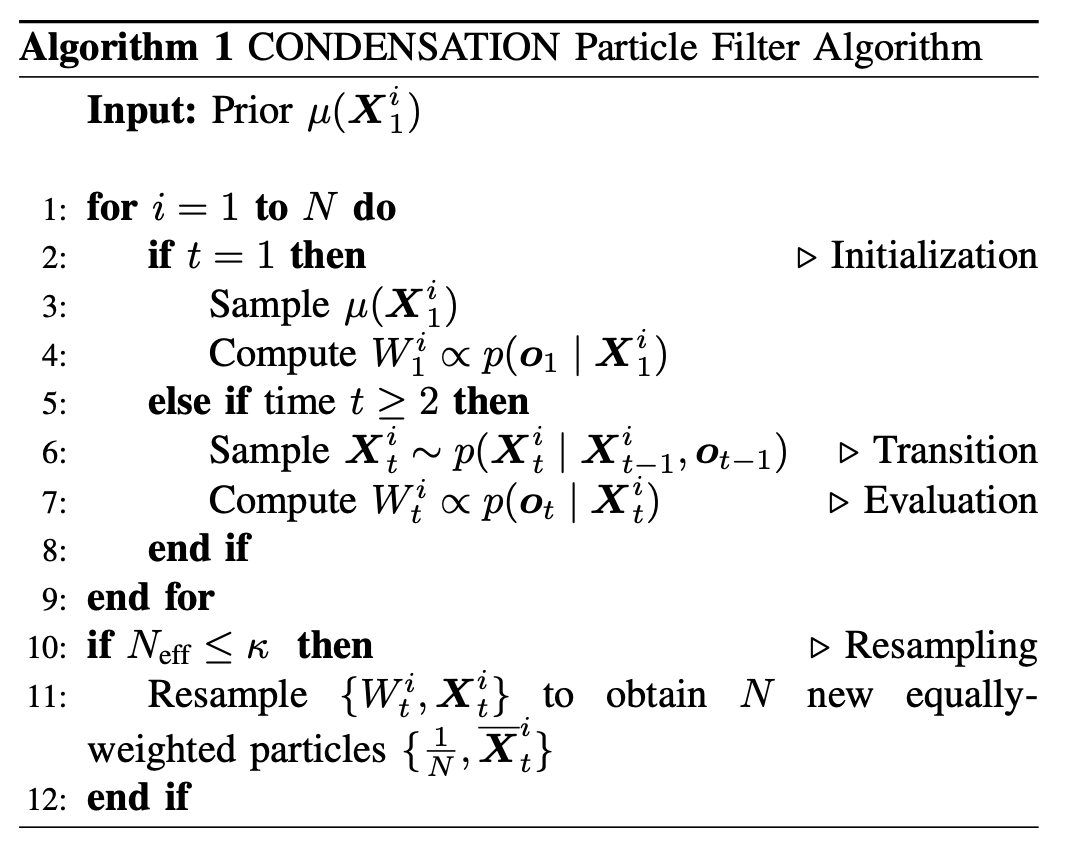
\includegraphics[width=90mm]{figs/condensation-algorithm.png}}
%\caption{Condensation Particle filter algorithm from \cite{b1}.}
%\label{fig:condensation-algorithm}
%\end{figure}


%0. Physics of ball? Also using it for the state transition model later. \\
%1. Simple Math Notations used for Kalman filter \\
%2. Simple Math Notations usef for Particle Filter \\
%3. Somehow introducing the boundaries to Particle Filter math? \\


\section{Results}

First we look into the estimation of the Kalman filter. 
\begin{figure}[h]
\centerline{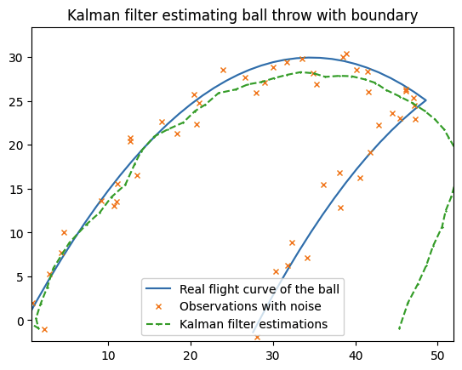
\includegraphics[width=90mm]{figs/kalman-filter.png}}
\caption{Kalman filter estimating ball throw with boundary. From own calculations.}
\label{fig:kalman-filter}
\end{figure}

In fig. 1 we can observe the Kalman filter trying to estimate the non-linear ball trajectory with a linear function, which results in bad estimations after the ball hit the wall, as expected. 

\begin{table}[htbp]
    \caption{Kalman filter estimation errors. Boundary 50 m away.}
    \begin{center}
    \begin{tabular}{|c|c|c|}
    \cline{1-3}
    & Before hitting the wall & After hitting the wall \\
    \cline{1-3} 
    Error & \textit{1.2 m} & \textit{17.73 m} \\
    \hline
    \end{tabular}
    \label{tab1}
    \end{center}
\end{table}
Next we explore the estimations of the Particle filter with low variance and a reasonable amount of observations.

\begin{figure}[h]
\centerline{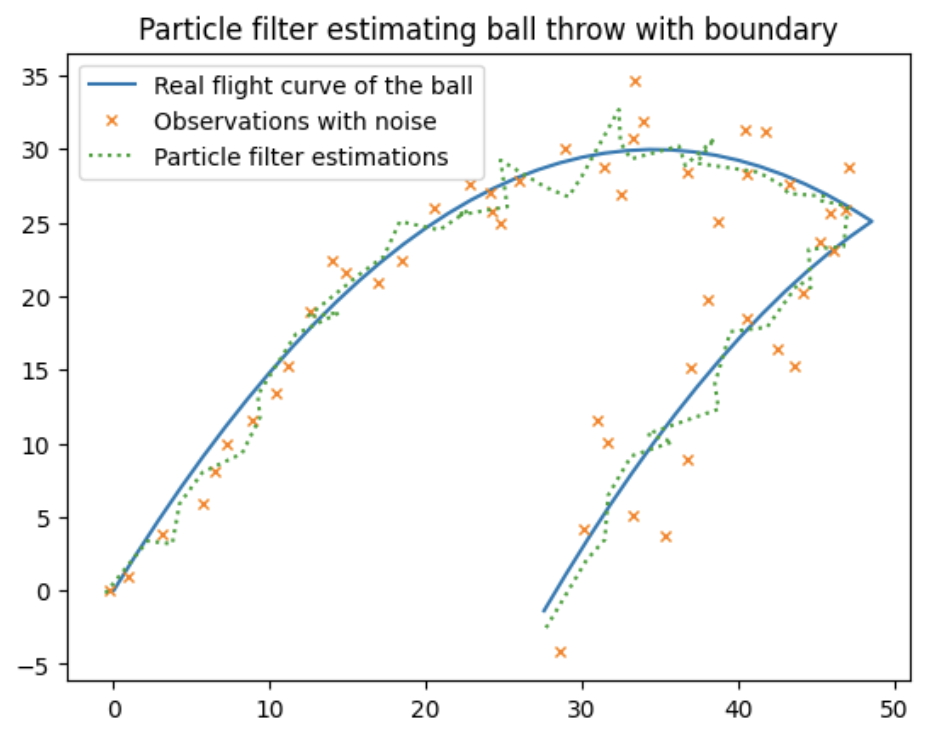
\includegraphics[width=90mm]{figs/particle-filter-knowing.png}}
\caption{Particle filter estimating ball throw with boundary. From own calculations.}
\label{fig:particle-filter-knowing}
\end{figure}

In fig. \ref{particle-filter-knowing} we can see that the Particle filter models the non-linear ball throw very well, as expected.
\begin{table}[htbp]
    \caption{Particle filter estimation errors. Boundary 50 m away. Boundary known in state transition.}
    \begin{center}
    \begin{tabular}{|c|c|c|}
    \cline{1-3}
    & Before hitting the wall & After hitting the wall \\
    \cline{1-3} 
    Error & \textit{1.87 m} & \textit{3.01 m} \\
    \hline
    \end{tabular}
    \label{tab1}
    \end{center}
\end{table}

To test the robustness of the Particle filter, we next drastically decrease the number of time steps.
\begin{figure}[h]
    \centerline{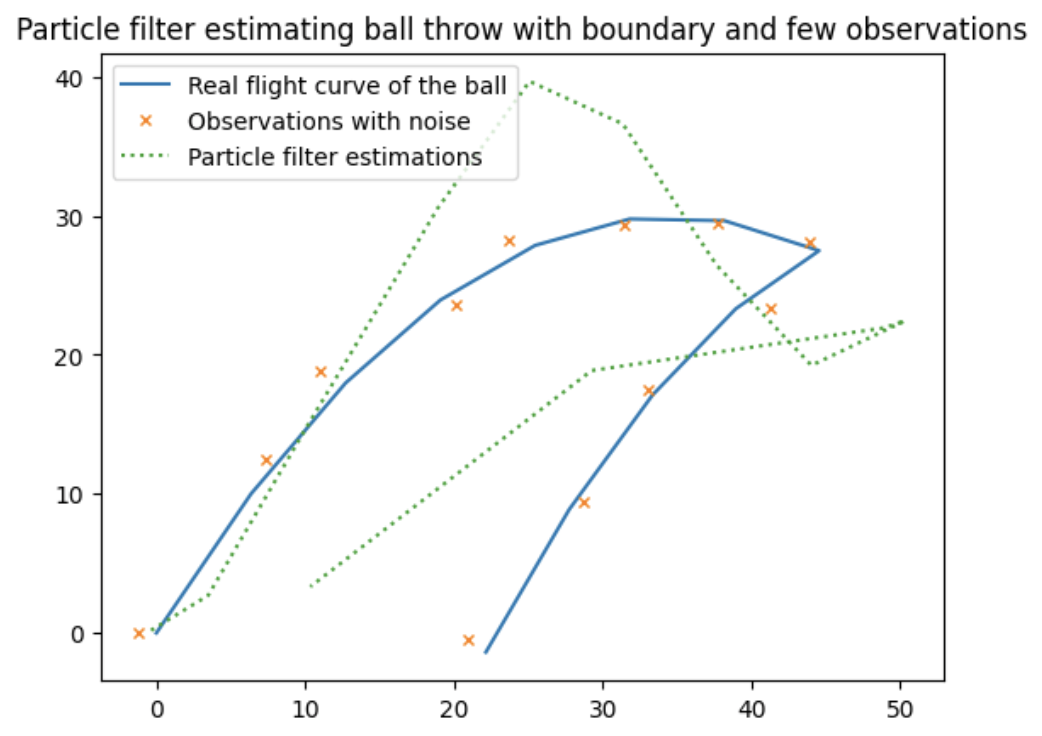
\includegraphics[width=90mm]{figs/particle-filter-few-observations.png}}
    \caption{Particle filter estimating ball throw with boundary and few observations. From own calculations.}
    \label{fig:particle-filter-few-observations}
\end{figure}
From fig. \ref{fig:particle-filter-few-observations} it is clear that the Particle filter has problems estimating the positions with these circumstances.
Although it is interesting to note that the general direction change can be modelled even though the observations are so few. \\
% TODO: Will ich hier auch die Table mit den Errors?
The second variable the Particle filter should be robust to is the variance of the observations to the real the trajectory.
\begin{figure}[h]
    \centerline{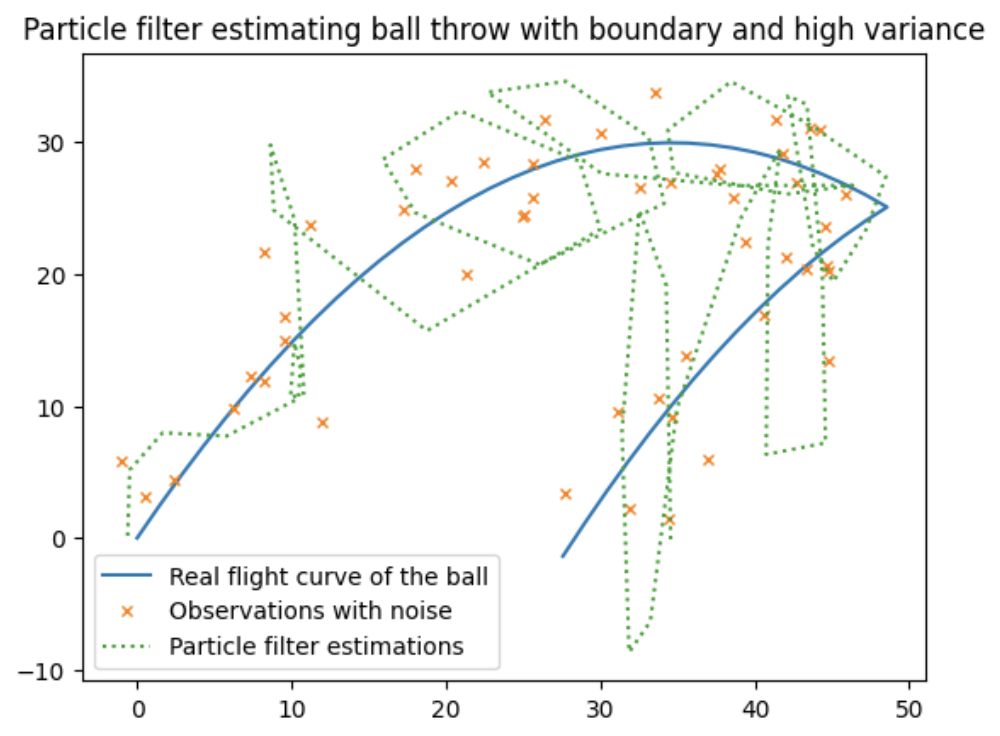
\includegraphics[width=90mm]{figs/particle-filter-high-variance.png}}
    \caption{Particle filter estimating ball throw with boundary and high variance. From own calculations.}
    \label{fig:particle-filter-high-variance}
\end{figure}
Although Particle filter also has a problem estimating the positions when the observations have high variance, as seen in fig. \ref{fig:particle-filter-high-variance}, the direction change after the ball hitting the wall is also generally modelled in this case.





% TODO
%1. Result of kalman filter handling the boundary \\
%2. Result of Particle filter handling the boundary with "known system dynamics" for the state transition \\
%3. Result of Particle filter handling the boundary without knowing the system dynamics/ knowing of the boundary \\

\section{Discussion}
% TODO: It makes sense that the general direction change is correctly modelled by the Particle filter since the wall is known in the state transition.
% For further study it would be interesting to see how the Particle filter would behave if the direction change after hitting the wall was not known in the state transition.
% In that case the Particle filter is not expected to be able to model direction change.

% The general robustness was not effected by the direction change, since these would also hold when the direction change would not be there. 

1. We see that the kalman filter is not able to apply for this "non-linear" problem. Because Kalman filter expects linear relations. Maybe an advanced Kalman filter would be applicable. \\
2. We see that Particle filter with knowledge of boundary can handle it quite nicely.  \\
3.  What we see for Particle filter without knowledge of boundary. \\

\section{Conclusion}

It would be interesting to see whether an advanced form of the kalman filter would be able to handle this non-linearity. 
- Naming which kind of kalman filter would be able to do it probably.
Other than that we could look at the particle filter, additionally not knowing the system dynamics in the state transition at all (now it just doesn't know of the boundary).




\section*{References}

Please number citations consecutively within brackets \cite{b1}. The 
sentence punctuation follows the bracket \cite{b2}. Refer simply to the reference 
number, as in \cite{b3}---do not use ``Ref. \cite{b3}'' or ``reference \cite{b3}'' except at 

\begin{thebibliography}{00} % TODO
\bibitem{b1} Fetzer, T., Bullmann, M., Ebner, M., Kastner, S., Deinzer, F., \& Grzegorzek, M. Interacting Multiple Model Particle Filter for Indoor Positioning Applications.
\bibitem{b2} Thrun, S. (2002). Probabilistic robotics. Communications of the ACM, 45(3), 52-57. % TODO: Correct?
\bibitem{b3} Isard, M., \& Blake, A. (1998). CONDENSATION--conditional density propagation for visual tracking. International journal of computer vision, 29(1), 5.
    
%\bibitem{b1} G. Eason, B. Noble, and I. N. Sneddon, ``On certain integrals of Lipschitz-Hankel type involving products of Bessel functions,'' Phil. Trans. Roy. Soc. London, vol. A247, pp. 529--551, April 1955.
\end{thebibliography}

\end{document}
